% ============================================== %
% PROPOSED METHODS %
% ============================================== %


\section{The D{i}VE Schemes}
\label{sec:dive_schemes}

%As discussed in Sec. ~ \ref{introduction}, the current view recommendations \cite{Vartak2014, Vartak2015, Ehsan2016} generated solely on the basis of importance score suffer from the redundancy problem. 

%\mas{new preamble}
In this section, we present our DiVE schemes for recommending diversified top views, which is captured by Eq.~\ref{objectif_function}, while at the same time minimizing the incurred processing costs.
%
Towards this, we first simply expand on the well-known {\em Greedy} heuristic for data diversification and propose our DiVE-Greedy scheme (Sec.~\ref{subsec:dive-greedy}). 
%
In Sec.~\ref{dive-greedy-static}, we propose novel pruning strategy that allows improving the efficiency of DiVE-Greedy. 
%
To overcome the {\em constructive} nature of DiVE-Greedy and allow better performance, we propose our {\em interchange} method DiVE-Swap in sections ~\ref{subsec:dive-swap} and ~\ref{subsec:dive-dswap}.
%
Finally, we introduce our {\em adaptive} pruning method, which is based on {\em non-parametric predictive intervals} and strikes a fine balance between  efficiency and effectiveness. 

\subsection{Baseline Solutions}\label{subsec:baseline}

As baseline solutions to compare the performance of our proposed DiVE schemes, we simply incorporate methods from existing work that optimize either for importance or diversity. 
% 
In terms of diversity, we employ the classical {\em Greedy Construction} algorithm \cite{Smyth2001}, which has been shown to maximize diversity within reasonable bounds compared to the optimal solution \cite{Yu2009, Vieira2011}. 
%
In this work, we refer to that baseline as {\em Greedy-Diversity}. 
%
Similarly, in terms of importance, we adopt the work on {\tt SeeDB} for recommending the top-k views with the highest deviation \cite{Vartak2015, Vartak2014}.
%
Particularly, in that method, all possible target and reference views are generated by executing their underlying queries, then the list of views is linearly scanned to recommend the top-k for which the target view shows high deviation from its corresponding reference view (denoted as {\em Linear-Importance} in this work).
%

Clearly, those two methods are ``oblivious" to our hybrid objective function (i.e., Eq.\ref{objectif_function}). 
%
%In particular, as shown in our experimental evaluation, each of those two methods performs well under extreme settings of our hybrid function.
%
Moreover, as expected and shown in our experimental evaluation, Greedy-Diversity provides its best performance when $\lambda=1.0$ (i.e., all preference is given to diversity), whereas Linear-Importance is the winner when $\lambda=0.0$ (i.e., all preference is given to importance). 
%
Next, we present our DiVE schemes which are able to provide the best performance, irrespective of the value of $\lambda$.



\subsection{The DiVE-Greedy Scheme}\label{subsec:dive-greedy}

\setlength{\textfloatsep}{0pt}% Remove \textfloatsep
\begin{algorithm}[t]
	\SetAlgoLined
	\KwIn{Set of views V and result set size k }
	\KwOut{Result set $ S \geq V $, |S| = k}  
	$S \leftarrow \left[V_i, V_j\right] $ get  two most distant views\;
	$X \leftarrow  \left[V \backslash S\right]$\;
	$i \leftarrow len\left(S\right) $\;
	\While{|S| < k}{
		%		\If{Pruning = True}{
		%			$ enablePruning $\;
		%		}
	%	\For{$j$ in set $X$}{
		%	$ max_v \leftarrow argmax F\left(X\left[j\right],S\right) $\;
		$ v_i \leftarrow argmax \left(1-\lambda\right) \times I\left(v_i\right) + \lambda \times setDist\left(v_i, S\right)$\;
	%	}
		$ S.add\left(v_i\right) $\;
		$ X.remove\left(v_i\right)$\;
	%	$ i  \leftarrow  i + 1 $\;
	}
	return S
	\caption{\textit{DiVE} Greedy}
	\label{DiVE-Greedy}
\end{algorithm}

In this section, we discuss our first DiVE scheme ({\em DiVE-Greedy}), which simply extends the basic Greedy Construction algorithm to work under our hybrid objective function (i.e., Eq.~\ref{objectif_function}). 
%
Such extension is straightforward  and is described in Algorithm \ref{DiVE-Greedy}. 
%
Similar to the classical Greedy Construction, DiVE-Greedy initializes the set $S$ with the two most distant views,  where the distance between any two views is calculated using our context-based function, as given in Eq.\ref{diversity_score}.
%
Then, DiVE-Greedy iteratively selects new views to be added to $S$. 
%
Particularly, in each iteration a view is selected from the set of remaining views $X$ and is added to $S$.
%
To make that selection, DiVE-Greedy assigns a score to each view in $X$, which is based on the hybrid objective function $F\left(S\right)$, as defined in equation \ref{objectif_function}. 
%
Specifically, the utility score assigned to a view $V_i \in X$ is computed as: 
\begin{equation}
	U\left(V_i\right)= \left(1-\lambda\right) \times I\left(V_i\right) + \lambda \times setDist\left(V_i, S\right)
	\label{utility_each_candidate}
\end{equation}
\noindent where $setDist\left(V_i, S\right) = \dfrac{1}{|S|} \sum_{\underset{V_j \in S}{j=1}}^{|S|} D\left(V_i, V_j\right) $
%\note{
Thus, in each iteration, the view with highest utility score is selected and added to $S$, until $|S|=k$, as shown in Algorithm \ref{DiVE-Greedy}.  
%}

\noindent {\bf DiVE-Greedy Cost:} 
%
Notice that the only difference between DiVE-Greedy and our baseline Greedy-Diversity (i.e., the classical Greedy algorithm) is in the utility score assigned to each view (i.e., $U(V_i)$ in Eq.\ref{utility_each_candidate}). 
%
In fact, in the special case where $\lambda=1.0$, Eq.~\ref{utility_each_candidate} boils down to $U\left(V_i\right)= setDist\left(V_i, S\right)$, which is the same score used by Greedy-Diversity for maximizing diversification. 
%
However, that simple change in the utility score leads to executing the query underlying each view $V_i$ in order to compute the $\left(1-\lambda\right) \times I\left(V_i\right)$ component of its score. 
%
Hence, the overall cost of DiVE-Greedy is $C_T=C_Q+C_D$, as opposed to the cost of Greedy-Diversity, which is only $C_T=C_D$, where $C_Q$ is the query processing cost (i.e., data-driven), and $C_D$ is the cost for computing Jaccard distances (i.e., query-driven), as described in Sec. ~\ref{sec:diversifying_recommended_visualizations}.

Clearly, $C_Q$ is equal to the number of possible views and is $O(n)$, where $n$ is the number of possible views, whereas $C_D$ is $O(kn)$, where $k$ is the number of recommended views.
%
Hence, as presented, our extended DiVE-Greedy is an instance of what has been described earlier as a "process-first-diversity-next" approach \cite{Zhang2008,Rafiei2010}, in which diversification only takes place after all possible views are executed to calculate their importance. 
%
In the next section, we describe our work to overcome the limitations of that approach.

\subsection{DiVE-Greedy with Pruning}\label{dive-greedy-static}

As mentioned in the previous section, the cost of the DiVE-Greedy algorithm is dominated by the query processing cost $C_Q$ and is proportional to the number of possible views. 
%
Although hundreds of views are generated for a given subset of data $D_Q$, only a small fraction of those views are actually of interest and are candidates to be included in the top-k set. 
%
As such, a significant fraction of the query processing cost is incurred in evaluating low-utility views. 
%
This observation motivated us to propose a pruning technique to minimize the search space of views and narrow it down to the most promising ones, as follows. 

\eat{%HAK version
As mentioned in the previous section, the cost of the DiVE-Greedy algorithm is dominated by the cost of executing view queries and is proportional to the number of possible views. 
%
Although hundreds of views are possible for a given subset of data, only a small fraction of the views are actually of interest and are included in the top-k set. Consequently, a significant fraction of the query processing cost is incurred on evaluating low-utility views. Hence, in this section we propose a pruning technique to reduce the search space of views. 
}


Our proposed pruning technique is based on the observation that the utility score of each view $U(V_i)$ is a weighted sum of two measures; 1) the importance score of the view (i.e., $I(V_i)$), and 2) the distance of the view from $S$ (i.e., $setDist\left(V_i, S\right) $). 
%
We note that the computation of $setDist\left(V_i, S\right)$ is a CPU-bound requires fast operation. 
%
To the contrary, computing the importance score of a view $I(V_i)$ is an expensive operation that requires executing two queries to generate the target and reference data for $V_i$.
%\mas{is max-min something we proposed or we borrowed from somewhere else? and is max-min a technical term?}\note{I think the technical term used in literature is branch and bound method, max-min is just used here. Should we change it to branch and bound?}
Thus, we employ a {\em max-min} pruning technique, that leverages the diversity score to bound the maximum utility score achieved by each view $V_i$, and in turn allows for pruning low-utility views without incurring the high cost for evaluating their importance.

\eat{%hak version
Our proposed pruning technique is based on the observation that the utility score of each view $U(V_i)$ is a weighted sum of two measures; 1) the importance score of view $I(V_i)$ and 2) distance of a view from S $ setDist\left(V_i, S\right) $. The computation of $ setDist\left(V_i, S\right)$ requires only CPU computations and is a faster operation. Whereas, computing the importance score of a view is an expensive operation that requires executing view query on both the target and reference subset of data. Thus, we employ a max-min pruning technique as presented in \cite{Khan2015}, that leverages the diversity score to estimate the utility score of a view without computing the importance score.}

%\begin{figure}
%	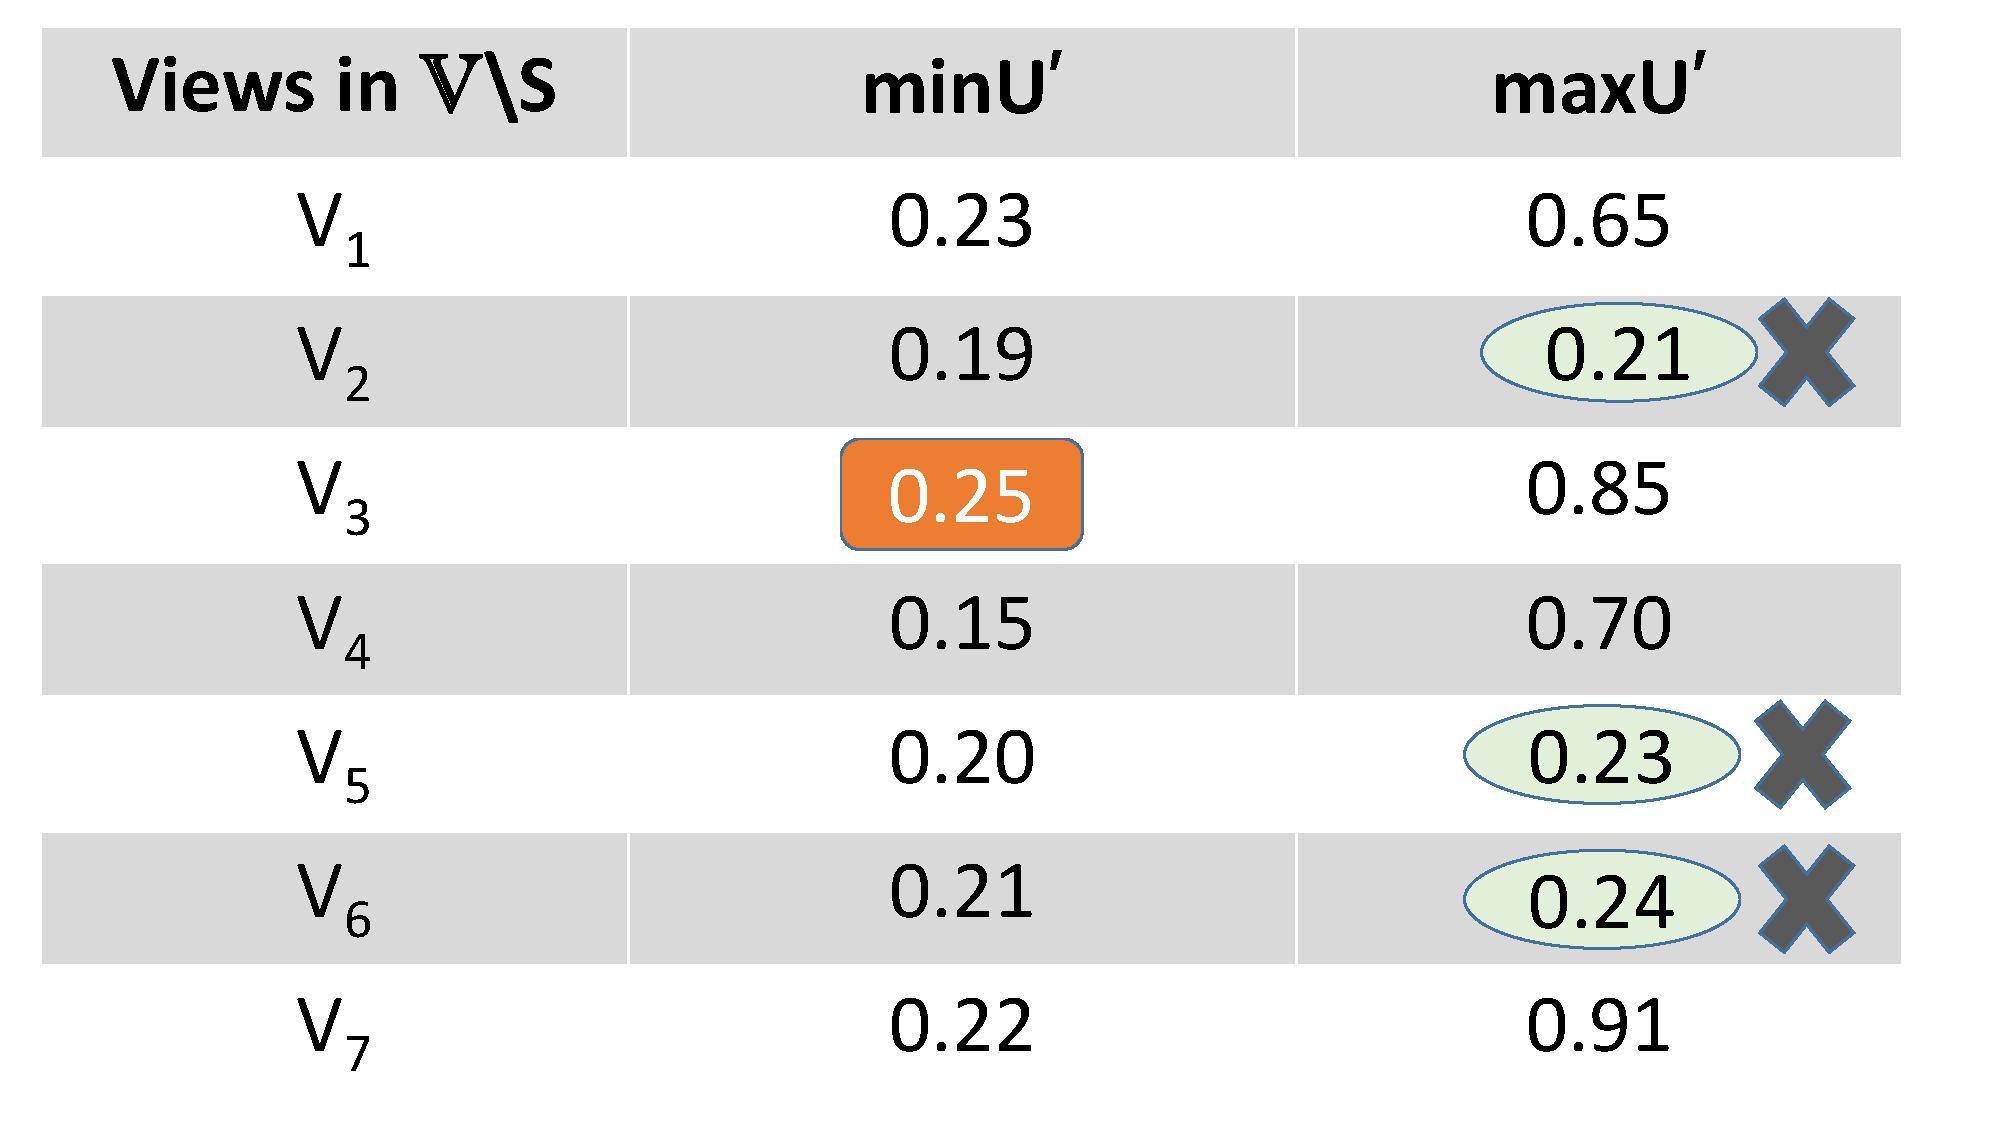
\includegraphics[width=3in]{figures/results/Max-Min}
%	\caption{Max-Min Pruning: All views which has $ maxU' $ less than the maximum of $ minU' $ will be pruned}
%	\label{fig:Max-Min}
%\end{figure}

Particularly, max-min utilizes the maximum and minimum bound on the importance score $I(V_i)$. 
%
%\mas{discuss bound}\note{you mean why the upper bound is $\sqrt{2}$}
Clearly, the minimum utility score is $I_0 = 0$, whereas the maximum utility value $I_u$ a view can score is computed as $I_u = \sqrt{2}$ (Sec. ~\ref{subsec:problem_definition}). 
%
Using those bounds, in each iteration the maximum $maxU(V_i)$ and minimum utility $minU(V_i)$ score for each view $V_i \in X$ is calculated as:
\[
 	maxU\left(V_i\right)= \left(1-\lambda\right) \times I_u\left(V_i\right) + \lambda \times setDist\left(V_i, S\right) 
\]
%\bigskip
\[	
minU\left(V_i\right)= \left(1-\lambda\right) \times I_0\left(V_i\right) + \lambda \times setDist\left(V_i, S\right) 
\]
Accordingly, the maximum value of $minU$ is recorded. 
%
Then, if $maxU$ of any candidate view is less than the maximum of $ minU$, then that view is pruned. 
%
%
%\mas{example is too simple - i think should be deleted} \note{both figure and text should be deleted or just text?}
%Figure \ref{fig:Max-Min} shows one simple iteration in which, the maximum value of $minU$ is $0.25$. 
%%
%Hence, all the views with $maxU$ value less than $0.25$ are pruned without executing their corresponding queries.
%%
%Once the actual importance score is calculated for the remaining views, then the view with highest utility score is selected and added to $S$.



\eat{ %hak version
The Max-Min pruning technique utilizes the maximum and minimum bound on the importance score. The maximum utility value $I_u$ a view can score is computed as $I_u = \sqrt{2}$,  and the minimum utility score is $I_0 = 0$. Using those bounds, in each iteration maximum and minimum utility score is calculated for each view in X as :
}

\eat{%hak version
\[
 	maxU'\left(V_i\right)= \left(1-\lambda\right).I_u\left(V_i\right) + \lambda.setDist\left(V_i, S\right) 
\]
%\bigskip
\[	
minU'\left(V_i\right)= \left(1-\lambda\right).I_0\left(V_i\right) + \lambda.setDist\left(V_i, S\right) 
\]

The maximum value of the $minU$ is recorded. If $maxU'$ of any candidate view is less than the maximum of $ minU'$, then that view is pruned. As shown in Figure \ref{fig:Max-Min}, the maximum value of $minU'$ is $0.25$. Hence, all the views with $maxU'$ value less than $0.25$ are pruned and view queries are generated only for the remaining views. Once the actual importance score is calculated for the remaining queries, the DiVE-Greedy algorithm selects the view with highest utility score to be added in S. Thus, the set of views computed by DiVE-Greedy using pruning is same as the one calculated without pruning.
}

\setlength{\textfloatsep}{0pt}% Remove \textfloatsep
\begin{algorithm}[t]
	\SetAlgoLined
	\KwIn{Set of views V and result set size k }
	\KwOut{Result set $ S \geq V $, |S| = k}  
	$S \leftarrow $ Result set of importance or diversity maximized\;
	$X \leftarrow  \left[V \backslash S\right]$\;
	\While{improve = True}{
		%		\If{Pruning = True}{
		%			$ enablePruning $\;
		%		}
		\For{$i$ in set $X$}{
			$ S' \leftarrow S $\;
			\For{$j$ in set $S$}{
				\If{ $ F\left(S'\right) < F\left(S \backslash S[j] \cup X[i]\right) $}{
					$ S'  \leftarrow S \backslash j \cup X[i] $  \;
				}
			}
			\If{ $ F\left(S'\right) > F\left(S\right) $}{
				$ S  \leftarrow S'$
			}
		}
%		\eIf{ $ F\left(S\right) > F_{current} $}{
%			$ F_{current}   \leftarrow F\left(S\right) $\;
%			$  improve \leftarrow  True $\;
%		}{
%		$  improve \leftarrow  False $\;
%	}
}
return S
\caption{\textit{DiVE} Swap}\label{DiVE-Swap}
\end{algorithm}


%
%This leads to two extreme baseline solutions, one based only on the importance score of the views which is called \textbf{\textit{"Linear-Importance"} } and second based on only diversity score of the views which is called \textbf{\textit{"Greedy-Diversity"}}. 
%
%Instead of uses one of those two extrem, \textit{DiVE} scheme employed hybrid function for evaluating top-k views which captures both the importance as well as diversity. Moreover, DiVE also equipped with pruning scheme which can prune a large number of queries without reducing the quality of the result. Our proposed DiVE scheme described below. 


%In order to capture both importance and diversity in the recommended top-k views, \textit{DiVE} employs a greedy construction algorithm to iteratively select views that maximize the hybrid objective function $F\left(S\right)$ as presented in equation 3, and it is called as \textbf{\textit{DiVE-Greedy}} scheme. 
%
%The details of the \textit{DiVE-Greedy} scheme are given in Algorithm \ref{DiVE-Greedy}. 
%%
%The key ingredient of any Greedy algorithm for solving an optimization problem is the objective function itself that needs to be maximized. In particular, \textit{DiVE-Greedy} initializes the set S with two most distant views. The distance between all the views is calculated using the distance function as given in equation 2. 
%%
%In each iteration, a new candidate view is selected from remaining views X and added to S. 
%
%Thus, \textit{DiVE-Greedy} assigns a utility score to each candidate view which is based on the hybrid objective function $F\left(S\right)$ as defined in equation \ref{objectif_function}. 
%
%The utility score of each candidate view $V_i$ in X is computed as: 
%
%\begin{equation}
%U\left(V_i\right)= \left(1-\lambda\right).I\left(V_i\right) + \lambda.setDist\left(V_i, S\right)
%\label{utility_each_candidate}
%\end{equation}
%
%Where $ setDist\left(V_i, S\right) = \dfrac{1}{|S|} \sum_{\underset{V_j \in S}{j=1}}^{|S|} D\left(V_i, V_j\right) $
%\newline
%
%Thus, the view with highest utility score in each iteration is selected and added to S.
%
%%\textit{DiVE-Greedy scheme costs.} There are four types of costs that required to run \textit{DiVE} scheme, as follows:
%%
%%\begin{itemize}
%%	\item Query cost $C_Q$: Cost that needed for the query execution, the cost of $C_Q$ depends on the query itself and the number of rows (tuples) of the dataset. This cost depends on CPU and I/O cost but it dominated by I/O costs. 
%%	\item Deviation/importance cost $ C_I $: The deviation computation cost is relatively cheap due to this cost only compute the probability distribution of each view and calculate the distance between two probability distribution of views (target view and reference view). The deviation equation can be seen in equation 1. This cost only from CPU costs.
%%	\item Diversity cost $C_D$: Cost which required not only the computation of dissimilarity between two context views but also for whole diversity computation. This cost also only from CPU costs. $C_D$ depends on the number of views and the diversity algorithm that used, e.g. Greedy construction is cheaper than Swap, the cheapest is Random Algorithm. 
%%	\item Visualization cost $C_V$: Cost which needed for plotting visualization and it only depends on CPU cost. 
%%\end{itemize}


%
%The costs of Greedy Construction algorithm has two components which are the query execution cost $C_Q$ that computing the importance score of view and the diversity cost $C_D$ that computing set distance of each view from the views already in S. The complexity of query execution cost is $ O$($n$) as the content of each view is generated only once. Meanwhile, the diversity cost $C_D$ is $ O$($kn$) where k is the size of subset of views S and $ n $ is the number of all possible views.
%
%Traditional diversification method applied approach such "process-first-diversity-next" which leads to generating all possible views and computing the importance score in advance, then the diversity is executed next. Although, greedy algorithm is very ent, however, as the number of attributes $\mathbb{A}$, measures $\mathbb{M}$ and aggregate functions $\mathbb{F}$ increase, the number of views that need to be generated grows exponentially. Hence, without a good strategy, \textit{DiVE-Greedy} suffers from the high costs of query execution. 
%
%Therefore, to overcome this issue, \textit{DiVE-Greedy} employs static pruning strategy as elaborated next. 
